\documentclass[10pt,twocolumn]{article}
\usepackage[margin=0.6in,top=0.55in,bottom=0.55in]{geometry}
\usepackage{amsmath,amssymb}
\usepackage{booktabs}
\usepackage{graphicx}
\usepackage[font=small,skip=3pt]{caption}
\usepackage{hyperref}
\usepackage{enumitem}
\usepackage{microtype}
\usepackage{titlesec}
\usepackage{url}
\usepackage{setspace}
\setstretch{0.9}

\titlespacing*{\section}{0pt}{4pt}{1.5pt}
\titlespacing*{\subsection}{0pt}{2.5pt}{0.5pt}
\titlespacing*{\paragraph}{0pt}{2pt}{0.6em}
\renewcommand{\arraystretch}{0.9}
\setlength{\columnsep}{14pt}
\setlength{\belowcaptionskip}{0pt}
\setlength{\textfloatsep}{6pt}
\setlength{\floatsep}{6pt}
\setlength{\intextsep}{6pt}
\setlength{\dbltextfloatsep}{6pt}
\setlength{\parskip}{0pt}
\abovedisplayskip=4pt \belowdisplayskip=4pt
\abovedisplayshortskip=2pt \belowdisplayshortskip=2pt
\predisplaypenalty=0
\raggedbottom

\hypersetup{colorlinks=true,linkcolor=blue,urlcolor=blue,citecolor=blue,
  pdftitle={AEGIS: Learning a Size-Invariant Interceptor Swarm for Drone Defense},
  pdfauthor={Abdul Samad Zaheer Khan}}

\newcommand{\vs}{\,v\,}

\begin{document}
\twocolumn[{%
\begin{center}
{\Large\textbf{AEGIS: Learning a Size-Invariant Interceptor Swarm for Drone Defense\\
with a Classical Allocator and One Shared PPO Policy}\par}
\vspace{0.9em}
{\normalsize Abdul Samad Zaheer Khan \quad
\small\texttt{ak9943@nyu.edu}\\[2pt]
\small November 2026\par}
\vspace{0.45em}
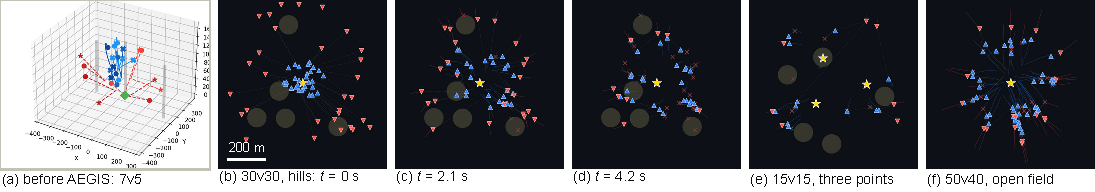
\includegraphics[width=\textwidth]{figures/replays.pdf}\\[1pt]
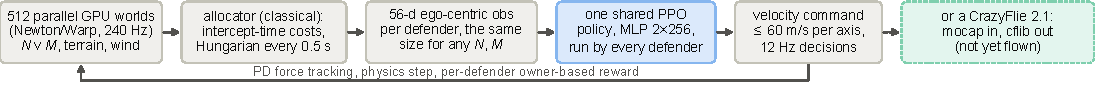
\includegraphics[width=\textwidth]{figures/pipeline.pdf}
\captionsetup{hypcap=false}
\captionof{figure}{(a)~Before AEGIS: end-to-end swarm RL, 7v5; no evaluation episode stopped every attacker. (b--d)~AEGIS,
30v30 raid in hills (\texttt{aegis\_big24}, trained up to 24v24): dotted lines are allocator assignments, crosses
eliminated drones. (e)~15v15, three points (\texttt{aegis\_vark}). (f)~50v40. Bottom: only the policy is learned.}
\label{fig:hero}
\end{center}
\vspace{0.1em}
}]
\thispagestyle{empty}

%% ---------------------------------------------
\begin{abstract}
\noindent
AEGIS trains a swarm of interceptor drones to defend one or more points against attack drones. End-to-end multi-agent
reinforcement learning (RL) with team rewards stalled at swarm scale: defenders piled onto the nearest attacker, and one
seven-defender run intercepted 3\%. In AEGIS a classical allocator assigns defenders to attackers by Hungarian matching on
intercept times, and one PPO policy, shared by every defender, flies each drone from a fixed-size, 56-d ego-centric
observation. It wins 98--100\% from 1v1 to 20v20 under hills, wind and noise, and \textbf{100\% at 50v40 and outnumbered
20v40} without training at those sizes; one checkpoint defends one to four points (95--100\%). Adversarial co-training
cut learned attackers' breach rate from 0.75 to 0.09. A CrazyFlie~2.1 deployment is verified in software but has not
yet flown.
\end{abstract}

%% ---------------------------------------------
\section{Task and history}

Defenders (60\,m/s) must destroy attackers (50\,m/s) before any reaches a protected point in a 1\,km\,$\times$\,1\,km
arena; team sizes $N$ and $M$, terrain (hills, urban blocks, mazes), raid type and wind are resampled every episode. A
\emph{win} means every attacker is destroyed and none breaches; \emph{realism} adds five hills, gusting wind, observation
noise and 300\,m detection. All numbers are fixed-seed simulation results.

Fig.~\ref{fig:timeline} traces the project. In March a SAC~\cite{sac} defender learned 1v1 interception; training then
moved to GPU physics (Warp~\cite{warp}, Newton~\cite{newton}), parameter-shared swarms and PPO~\cite{ppo},
and stalled (Fig.~\ref{fig:hero}a). A July audit blamed the task: team rewards plus a first-to-touch
bonus paid for piling on; a dead defender's zero reward shielded it from breach penalties; outcomes lay far beyond the
${\approx}2$\,s horizon of $\gamma{=}0.99$ at 48\,Hz; and a bug teleported the target whenever any of 1,024 parallel
worlds reset. AEGIS keeps learning only for flight and interception and moves coordination into a classical allocator;
all of Fig.~\ref{fig:results} followed within six weeks.

%% ---------------------------------------------
\section{Method}

\paragraph{Allocator.} In each world, alive defenders $d$ and detected attackers $a$ get costs
\begin{equation*}
C_{da} = t_\mathrm{go} + 100\,[t_\mathrm{go} > t_\mathrm{br} - 1\,\mathrm{s}] - u_a - 0.5\,[d \text{ owns } a]:
\end{equation*}
the closed-form intercept time, a penalty if $d$ would arrive after $a$ breaches, an urgency bonus
$u_a=\min(20/\max(t_\mathrm{br},0.5),10)$ and hysteresis. SciPy's Hungarian solver~\cite{kuhn} assigns; surplus defenders
double up or guard. Re-allocating every 0.5\,s and on any death, kill, breach or detection makes the swarm self-healing:
with two defenders killed mid-fight it still wins 98--100\%.

% Both floats are defined here, in the second column of page 1: the timeline goes to the top of that column and the
% results figure to the top of page 2 (LaTeX keeps figures in order, so the timeline must come first).
\begin{figure}[t]
\centering
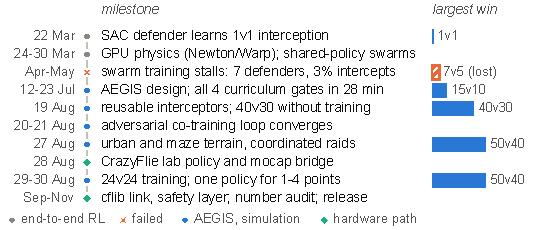
\includegraphics[width=\columnwidth]{figures/timeline.pdf}
\caption{Timeline, 2026; bars: largest engagement won.}
\label{fig:timeline}
\end{figure}

\begin{figure*}[t]
\centering
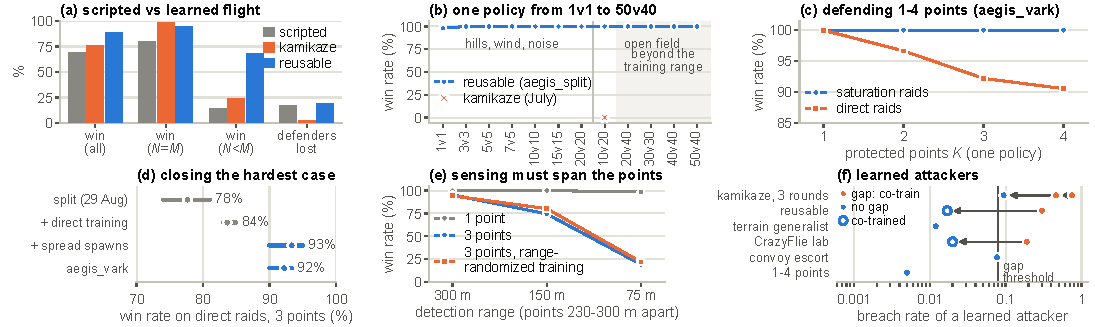
\includegraphics[width=\textwidth]{figures/results.pdf}
\caption{Results. (a)~Realism grid, 38 cells $\times$ 3 raids, $n{=}32$. (b)~\texttt{aegis\_split} (trained 6--20\vs3--20),
$n{=}100$ (realism) or 60 (open field) per cell and raid; cross: kamikaze policy. (c)~\texttt{aegis\_vark}, $n{=}60$.
(d)~Three points, direct raids: mean, range over 10v10--20v20. (e)~$n{=}48$. (f)~A new RL attacker's breach rate vs.\
each frozen defender; open: co-trained (threshold 0.10, later 0.08).}
\label{fig:results}
\end{figure*}

\paragraph{Policy and rewards.} One PPO MLP (two layers of 256; Stable-Baselines3~\cite{sb3}) runs on every defender. Its
56-d input (own state, the assigned attacker's relative state and predicted intercept point (PIP), nearest teammates,
obstacles and arena margins, the nearest other attacker) has the same size for any $N$ and $M$. It
commands velocity (${\pm}60$\,m/s) at 12\,Hz, tracked by a PD controller over 240\,Hz physics, with $\gamma{=}0.995$.
Rewards are per-agent and owner-based: potential-based shaping~\cite{ng} toward the assigned attacker, $+30$ per
intercept, $-30$ per crash ($-60$ for the champions), $-25$ to the owner of a breaching attacker ($-5$ to the others) and
$+10$ per team win; tests check that no exploit (hovering, pile-on, suicide, kill-stealing) pays better.

\paragraph{Training.} Up to 512 worlds run in parallel on one NVIDIA DGX Spark (159k--214k agent-steps/s); swept-segment
checks keep 110\,m/s closing speeds from tunnelling through the 3\,m intercept radius. Four gated stages, from 1v1
pursuit to 3--8\vs1--8 with terrain, wind, noise, jinking raids and random defender losses, passed in 28 minutes of
training; stage~3 alone did worse (win 0.72 vs 0.76, with six times the losses). Checkpoints are chosen by breach rate,
never by mean reward. Champions fine-tune with up to 24v24 teams, urban and maze terrain, coordinated raids and moving
or multiple targets.

%% ---------------------------------------------
\section{Results}

\paragraph{Learning vs.\ scripting (Fig.~\ref{fig:results}a).} With the same allocator, scripted flight to the PIP ties
the learned policy in all 114 entries of an open-field grid; under realism the policy lowers the breach rate in 67, ties
45, is worse in 2, and cuts defender losses from 17.4\% to 2.5\%. Kamikaze interceptors lose outnumbered cells by
construction; reusable ones (2\,s rearm) raised outnumbered wins from 24\% to 68\% and the exchange ratio from 0.98 to
8.97.

\paragraph{Size invariance (b).} \texttt{aegis\_split} wins 98\% at 1v1 and 100\% with zero leakers from 3v3 to 20v20
under realism (2--4\% defender losses), and 100\% with no losses at 30v30--50v40 and 20v40, sizes it never trained on.

\paragraph{Several points (c--e).} Defenders follow attackers, not points, so no allocator change was needed:
\texttt{aegis\_vark} wins 100/98/96/95\% for one to four points. Direct raids on three points rose from 74--81\% to
90--95\% with direct-weighted training and spawns spread over the points. Detection must span the points: at 150 and
75\,m, three points fall to 74\% and 19\% (one point: 98--100\%), and range-randomized training reaches only 80\% and
22\%.

\begin{figure}[t]
\centering
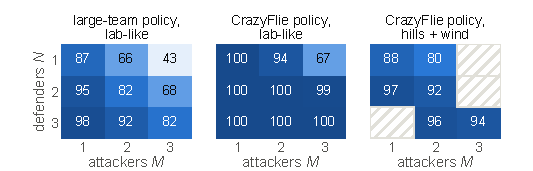
\includegraphics[width=\columnwidth]{figures/crazyflie.pdf}
\caption{Small-team win rate (\%): large-team champion vs.\ CrazyFlie policy (lab-like, $n{=}200$); the latter in
hills and wind ($n{=}100$).}
\label{fig:cf}
\end{figure}

\paragraph{Learned attackers (f).} RL attackers train against each frozen defender; above a breach threshold the defender
retrains against scripted raids plus the attacker pool~\cite{psro}. The first found \emph{kamikaze-baiting}, luring
pursuers into hills (win 0.78\,$\to$\,0.01); the loop shrank the exploit from 0.75 to 0.094 with no scripted regression.
Reusable defenders needed one round (0.30\,$\to$\,0.017), large-team policies warm-started from them showed no gap, and
only the small-team CrazyFlie policy needed another (0.19\,$\to$\,0.020).

%% ---------------------------------------------
\section{Toward hardware: CrazyFlie 2.1}


Scaling length by 1/125 and time by $\sqrt{2}$ maps the arena onto an 8\,$\times$\,8\,m lab (0.34\,m/s, policy at
8.49\,Hz, setpoints at 30\,Hz). The large-team champion is weak in small teams (Fig.~\ref{fig:cf}); a lab policy with
minimal sensing wins 100\% whenever $N\geq M$, and 88--97\% under unseen hills and wind. The bridge passes motion capture
through the same allocator and encoder (matching the simulator to $2{\times}10^{-5}$) and policy to cflib
velocity setpoints, behind a geofence and a stale-mocap watchdog; a 2v2 dry run intercepts both attackers by 4.1\,s.

%% ---------------------------------------------
\section{Limitations and lessons}

\textbf{Nothing has flown yet}; the simulator uses PD velocity tracking instead of rotor dynamics and shares detection
across the team. Attrition is the soft spot (5--12\% of defenders lost among obstacles); safety shaping and a speed brake traded hill losses for open-field ones. What worked: coordination in an
allocator that unit tests can verify, a fixed-size ego-centric view that carried one policy across team size, target
count and target motion, and gated stages, breach-based checkpoints, learned adversaries and an audit of every reported
number. The droneVdrone repository holds the code, logs and CSVs; \texttt{figures/make\_figures.py} rebuilds every figure.

\begin{thebibliography}{9}\scriptsize
\setlength{\itemsep}{0pt}\setlength{\parsep}{0pt}\setlength{\topsep}{1pt}
\bibitem{sac} T.~Haarnoja et al. Soft actor-critic: Off-policy maximum entropy deep reinforcement learning with a
stochastic actor. \emph{ICML}, 2018.
\bibitem{warp} M.~Macklin. Warp: A high-performance Python framework for GPU simulation and graphics. \emph{NVIDIA GTC},
2022.
\bibitem{newton} Newton contributors. Newton: GPU-accelerated physics simulation for robotics. GitHub, 2025.
\bibitem{ppo} J.~Schulman et al. Proximal policy optimization algorithms. arXiv:1707.06347, 2017.
\bibitem{kuhn} H.~W.~Kuhn. The Hungarian method for the assignment problem. \emph{Naval Res.\ Logistics Q.}, 2:83--97,
1955.
\bibitem{sb3} A.~Raffin et al. Stable-Baselines3: Reliable reinforcement learning implementations. \emph{JMLR}, 22, 2021.
\bibitem{ng} A.~Y.~Ng et al. Policy invariance under reward transformations: Theory and application to reward shaping.
\emph{ICML}, 1999.
\bibitem{psro} M.~Lanctot et al. A unified game-theoretic approach to multiagent reinforcement learning. \emph{NeurIPS},
2017.
\end{thebibliography}

\end{document}
